\documentclass{standalone}
\usepackage{tikz}
\usepackage{xcolor}

\begin{document}

\tikzset{
  c/.style={every coordinate/.try}
}

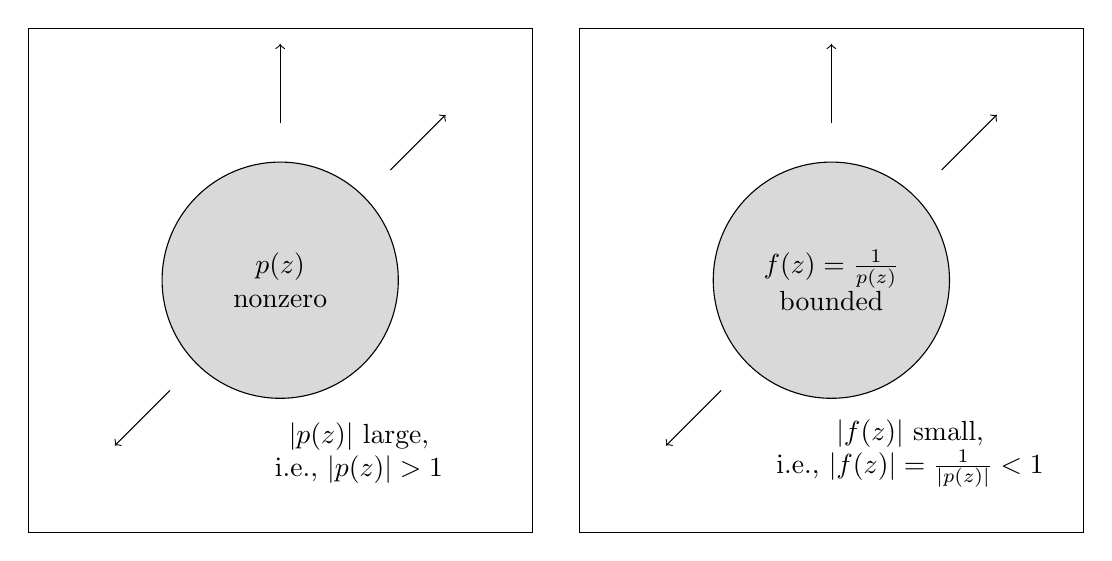
\begin{tikzpicture}
% box around sketch
\draw (3.2, 3.2) -- (-3.2, 3.2) -- (-3.2, -3.2) -- (3.2, -3.2) -- cycle;
% "small" compact region
\filldraw[fill=gray!30,draw=black,align=center] (0,0) node {$p(z)$ \\nonzero} circle (1.5cm);
\node[align=center] at (1, -2.2) {$|p(z)|$ large, \\i.e., $|p(z)|>1$};
% a bunch of arrows to show ... that it's bounded "out there"
%\draw[->] (2,0) -- (3,0);
\draw[->] (1.4,1.4) -- (2.1,2.1);
\draw[->] (0,2) -- (0,3);
%\draw[->] (-1.4,1.4) -- (-2.1,2.1);
%\draw[->] (-2,0) -- (-3,0);
\draw[->] (-1.4,-1.4) -- (-2.1,-2.1);
%\draw[->] (0,-2) -- (0,-3);
%\draw[->] (1.4,-1.4) -- (2.1,-2.1);

\begin{scope}[shift={(7,0)}]
	\draw (3.2, 3.2) -- (-3.2, 3.2) -- (-3.2, -3.2) -- (3.2, -3.2) -- cycle;
	\filldraw[fill=gray!30,draw=black,align=center] (0,0) node {$f(z)=\frac{1}{p(z)}$ \\bounded} circle (1.5cm);
	\node[align=center] at (1, -2.2) {$|f(z)|$ small, \\i.e., $|f(z)|=\frac{1}{|p(z)|}<1$};
	\draw[->] (1.4,1.4) -- (2.1,2.1);
	\draw[->] (0,2) -- (0,3);
	\draw[->] (-1.4,-1.4) -- (-2.1,-2.1);
\end{scope}
\end{tikzpicture}
\end{document}